% **************************************************************************** %
%                                                                              %
%                                                         :::      ::::::::    %
%    sec_resultados.tex                                 :+:      :+:    :+:    %
%                                                     +:+ +:+         +:+      %
%    By: acampo-p <acampo-p@student.42urduliz.com>  +#+  +:+       +#+         %
%                                                 +#+#+#+#+#+   +#+            %
%    Created: 2022/12/07 17:42:28 by acampo-p          #+#    #+#              %
%    Updated: 2023/02/12 17:57:38 by acampo-p         ###   ########.fr        %
%                                                                              %
% **************************************************************************** %

\section{RESULTADOS}

Una vez simulados los distintos escenarios,
se ha procedido a analizar las tablas de datos obtenidos por la simulación.

\begin{table}
	\centering
	\caption{Capacidad máxima de ensayos por maquina.}
	\documentclass[varwidth=\maxdimen]{standalone}
\usepackage[utf8]{inputenc}
\usepackage[spanish]{babel}
\usepackage{booktabs}

\begin{document}

\begin{tabular}{ l c }
	\toprule
	Ensayo & Capacidad máxima (unds.) \\
	\midrule
	\textit{Endurance}	& 934 \\
	\textit{Rolling Resistance}		& 2502 \\
	\bottomrule
\end{tabular}

\end{document}

	\label{tab:4_tbl_max_cap}
\end{table}

En la Figura~\ref{fig:4_hist_tests_done} se han graficado
las distribuciones de el numero de ensayos realizados, en un año simulado,
para cada escenario.
Cada escenario ha sido ejecutado 100 veces, y se ha trazado la frecuencia
con la que ocurría un determinado numero de ensayos en el histograma.
La figura consta de 2 gráficas,
correspondiendo el histograma (A) a los ensayos Endurance
y el histograma (B) a los ensayos Rolling.
De izquierda a derecha se pueden observar 4 distribuciones de distintos colores.
Cada uno de ellos corresponde a una configuración de turnos
del técnico encargado de estas maquinas.
Los turnos en los cuales el operario esta disponible como recurso
van desde 1 a tiempo completo, incluidos los fines de semana.

En el histograma superior puede observarse la distinción
que ocurre entre las distintas configuraciones.
Cada configuración tiene un amplio rango de ensayos,
mostrando el comportamiento estocástico de este tipo de ensayos.
Exceptuando la configuración a tiempo completo,
la cantidad de ensayos, parece variar dentro de un rango común de 100 ensayos.
Esta tendencia cambia al disponer a tiempo completo
de un operario que monte la maquina.
Al eliminarse la posibilidad
de que el ensayo finalice fuera del horario laboral,
la desviación estándar de ensayos realizados se reduce al mismo tiempo
que la media de ensayos se aproxima a la capacidad ideal.

En el histograma inferior,
las 3 primeras configuraciones expuestas,
muestran un comportamiento similar observado en
la configuración a tiempo completo, observada en el anterior gráfico.
Esto se debe, a que el técnico solamente puede llegar a lanzar
un determinado numero de ensayos por turno trabajado.
Esta cantidad se mantiene uniforme a lo largo de las ejecuciones
debido a que la duración de este ensayo es inferior
a la duración del turno del técnico.
Mientras el horario de trabajo sea limitado
la tendencia de ensayos corresponderá a la ecuación~\ref{eq:testdone}.
En el escenario en el que el técnico esta disponible durante 3 turnos al día,
la acumulación de eventos aleatorios se vuelve notable
en la desviación de ensayos observada respecto a los anteriores 2 escenarios.
Finalmente, a tiempo completo, la desviación estándar
aumenta considerablemente, ya que no hay un descanso
que regule la aleatoriedad de los ensayos.

\begin{equation}
	Test Realizados = 365 \cdot 8 \cdot 
	\underbrace{
		\left(\frac{N_{turnos}}{\mu_{test}} + 1\right)
	}_{\text{Entero truncado}}
	\label{eq:testdone}
\end{equation}

Una representación mas significativa ocurre
cuando se normaliza la cantidad de ensayos respecto
a la capacidad máxima de trabajo.
De esta marera, se obtiene la fracción de tiempo de utilización de maquina
representado en la Figura~\ref{fig:4_hist_time_sat}.
Esta conversión logra asentar la base necesaria para
comparar el grado de utilización de maquinas de manera directa.

\begin{figure}
	\begin{center}
		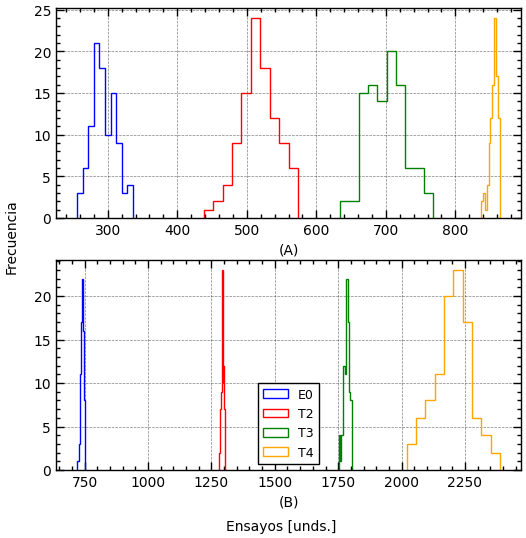
\includegraphics{fig/4_hist_tests_done}
	\end{center}
	\caption{Distribución de ensayos realizados para los escenarios descritos en la leyenda.
	(A) Ensayos endurance. (B) Ensayos rolling.}
	\label{fig:4_hist_tests_done}
\end{figure}

\begin{figure}
	\begin{center}
		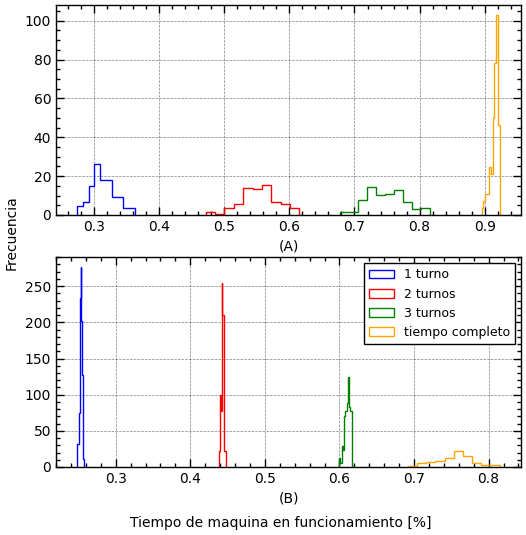
\includegraphics{fig/4_hist_time_sat}
	\end{center}
	\caption{Distribución de el nivel de saturación en tiempo de lo escenarios descritos en la leyenda.
	(A) Ensayos endurance. (B) Ensayos rolling.}
	\label{fig:4_hist_time_sat}
\end{figure}

\begin{table}
	\centering
	\caption{Media y desviación estándar de ensayos realizados por cada escenario y tipo de ensayo.}
	\documentclass[varwidth=\maxdimen]{standalone}
\usepackage[utf8]{inputenc}
\usepackage[spanish]{babel}
\usepackage{booktabs}
\usepackage{multirow}

\begin{document}

\begin{tabular}{ l c c c c }
	\toprule
	Escenario &
	\multicolumn{2}{c}{Ensayos \textit{Endurance} (unds.)} &
	\multicolumn{2}{c}{Ensayos \textit{Rolling Resistance} (unds.)} \\
		& $\mu$		& $\sigma$	& $\mu$		& $\sigma$ \\
	\midrule
	E0	& 293.35    & 17.27		& 739.35	& 5.51 \\
	T2	& 516.83	& 26.38		& 1293.40	& 5.00\\
	T3	& 701.07	& 27.25		& 1782.26	& 11.15 \\
	T4	& 855.06	& 5.70		& 2202.28	& 73.18 \\
	\bottomrule
\end{tabular}

\end{document}

	\label{tab:4_tbl_test_done}
\end{table}

Si se grafica la fracción de tiempo de utilización de maquina,
respecto a la fracción del tiempo trabajado,
con los escenarios expuestos hasta ahora,
se obtiene la Figura~\ref{fig:4_sctr_time_sat}.
La dispersión de los datos se ajusta perfectamente a una regresión lineal
a partir de la fracción de tiempo trabajado de 0.25 en adelante.
Para ambas maquinas, la relación entre ensayos realizados
y tiempo trabajado es directamente proporcional.
La obtención de esta relación,
junto con las capacidades máximas de las maquinas
expuestas en la tabla~\ref{tab:4_tbl_max_cap} permite 
anticipar si la capacidad del LCP será suficiente
para saciar la demanda de ensayos.

Teniendo en cuenta los datos obtenidos a través de la regresión lineal,
la ecuación~\ref{eq:qced} modela la cantidad de ensayos endurance
realizados en función a la fracción de horas trabajadas en un año.
Siendo la fracción de horas trabajadas descrita como la ecuación~\ref{eq:f_hours}.
A su vez, la ecuación~\ref{eq:rr} aplica la misma función
pero para los ensayos rolling.
Para un determinado objetivo de test realizados,
las ecuaciones mencionadas pueden resolverse
para obtener la cantidad de horas necesarias para llegar al objetivo.
En el caso de requerir más horas de las que una jornada laboral normal dispone,
se propone completar dichas horas sobrantes
reposicionando uno de los técnicos en un turno adicional durante un periodo.
Dicho periodo se puede calcular mediante la ecuación~\ref{eq:period},
de esta manera se aprovechan al máximo los recursos humanos disponibles.
Para ello primeramente se calcula
el máximo de turnos anuales mediante la ecuación~\ref{eq:gf}.

\begin{equation}
	Test Realizados = 934 \cdot 0.79 \cdot f_{t trabajo} + 0.15
	\label{eq:qced}
\end{equation}

\begin{equation}
	Test Realizados = 2502 \cdot 0.66 \cdot f_{t trabajo} + 0.12
	\label{eq:rr}
\end{equation}

\begin{equation}
	f_{t trabajo}= \frac{t_{trabajo}}{365~\frac{\text{días}}{\text{año}} \cdot
	24~\frac{\text{horas}}{\text{días}}}
	\label{eq:f_hours}
\end{equation}

\begin{equation}
	\begin{array}{c}
		G(f_{t trabajo}) = f_{t trabajo}
		\frac{365~\text{días}
		\cdot 24~\frac{\text{horas}}{\text{días}}}
		{8~\frac{\text{horas}}{\text{días}} \cdot
			5~\frac{\text{días}}{\text{semanas}} \cdot
		52~\frac{\text{semanas}}{\text{año}}} \\
		\\
		Turnos= 
		\begin{cases}
			1	& G(f_{t trabajo}) \leq 1 \\
			2	& 1 < G(f_{t trabajo}) \leq 2 \\
			3	& 2 < G(f_{t trabajo}) \leq 3 \\
			4	& G(f_{t trabajo}) > 3
		\end{cases}
	\end{array}
	\label{eq:gf}
\end{equation}

\begin{equation}
	Periodo = 12~\text{meses} \cdot (G(f_{t trabajo}) - Turnos -1)
	\label{eq:period}
\end{equation}

\begin{figure}
	\begin{center}
		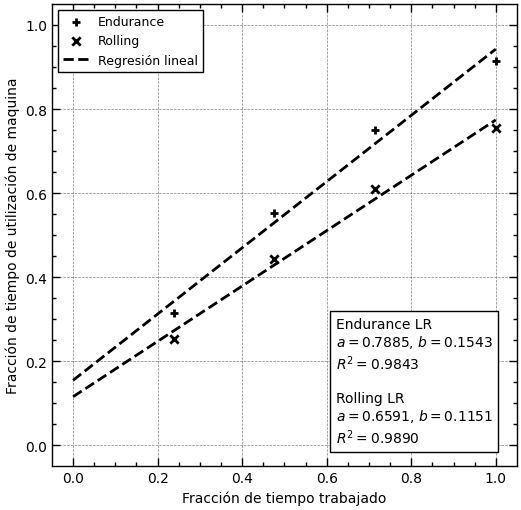
\includegraphics{fig/4_sctr_time_sat}
	\end{center}
	\caption{Tendencia proporcional del aumento del numero de ensayos al añadir turnos de trabajo.}
	\label{fig:4_sctr_time_sat}
\end{figure}

Con el fin de descartar otro tipo de configuraciones,
como múltiples técnicos trabajando simultáneamente,
se ha graficado la Figura~\ref{fig:4_box_techn1-2_comp}.
La diferencia en ambos ensayos parece mínima,
pero con la intención de descartar la idea de que
2 técnicos trabajando simultáneamente incrementa el numero de ensayos realizados,
se desarrolla el siguiente test de hipótesis.

\begin{itemize}
	\item $H_1$: $\mu_1 \neq \mu_2$
	\item $H_0$: $\mu_1 = \mu_2$
\end{itemize}

Se ha tratado de descartar la hipótesis nula mediante la prueba de valor-p,
y test t-student.
Los resultados de la prueba,
han sido recogidos en la tabla~\ref{tab:4_tbl_studet-t}.
El bajo valor-p obtenido en ambos tipos de ensayo
descarta la hipótesis nula formulada anteriormente.
Esto significa que las distribuciones
tienen una diferencia estadísticamente significativa.
A un siendo este el caso,
el escenario en el que se trabaja a 2 turnos,
es definitivamente superior,
como se puede observar en la Figura~\ref{fig:4_box_techn1-2_comp}.
Al consumir ambos la misma cantidad de recursos,
esto descarta la configuración en la que 2 técnicos trabajan simultáneamente.

\begin{table}
	\centering
	\caption{Resultados del test estadístico formulado a partir de los resultados de la Figura~\ref{fig:4_box_techn1-2_comp}}
	\documentclass[varwidth=\maxdimen]{standalone}
\usepackage[utf8]{inputenc}
\usepackage[spanish]{babel}
\usepackage{booktabs}
\usepackage{multirow}

\begin{document}

\begin{tabular}{ l c c }
	\toprule
	Resultados	& Endurance	& Rolling \\
	\midrule
	valor-t		& -2.279	& -5.179 \\
	valor-p		& 0.023		& 0.000 \\
	\bottomrule
\end{tabular}

\end{document}

	\label{tab:4_tbl_studet-t}
\end{table}

\begin{figure}
	\begin{center}
		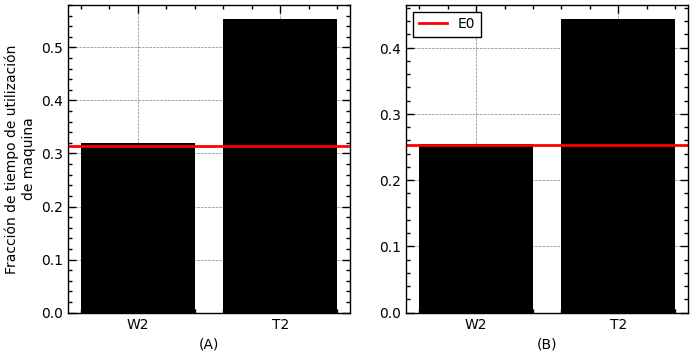
\includegraphics[width=\textwidth]{fig/4_bar_2shift-2techn_comp}
	\end{center}
	\caption{Comparación de el nivel de saturación en tiempo entre: [I] 2 técnicos trabajando simultáneamente, [II] 2 técnicos en distintos turnos.
	(A) Ensayos endurance. (B) Ensayos rolling.}
	\label{fig:4_bar_2shift-2techn_comp}
\end{figure}

\begin{figure}
	\begin{center}
		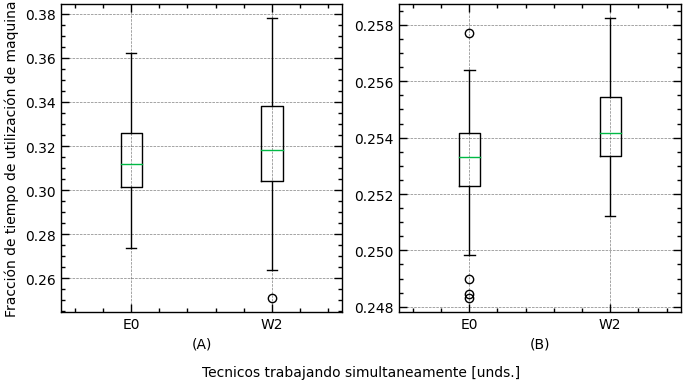
\includegraphics[width=\textwidth]{fig/4_box_techn1-2_comp}
	\end{center}
	\caption{Comparación de el nivel de saturación en tiempo entre 1 técnico y 2 técnicos trabajando simultáneamente.
	(A) Ensayos endurance. (B) Ensayos rolling.}
	\label{fig:4_box_techn1-2_comp}
\end{figure}

Por ultimo, se ha tratado de observar la en el rendimiento de ensayos
que aportaría la instalación de nuevas maquinas para el ensayo endurance.
En la Figura~\ref{fig:4_sctr_indoor}, se observa como añadir maquinas
no aumenta de manera significativa la cantidad de ensayos realizados,
ya que el técnico queda saturado de trabajo con la configuración actual.

Este análisis concluye, que en caso de necesitar capacidad adicional,
se opte por reposicionar a uno de los técnicos
en un turno adicional durante el periodo que sea necesario.
Ya que, es con diferencia la opción mas optima.

\begin{figure}[H]
	\begin{center}
	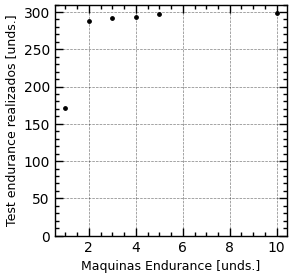
\includegraphics{fig/4_sctr_indoor}
	\end{center}
	\caption{Aumento de los ensayos realizados en función de las maquinas endurance instaladas.}
	\label{fig:4_sctr_indoor}
\end{figure}
